% Copyright (C) 2012  Dmitry V. Levin <ldv@altlinux.org>
% Permission is granted to copy, distribute and/or modify this document
% under the terms of the GNU Free Documentation License, Version 1.2
% or any later version published by the Free Software Foundation;
% with no Invariant Sections, no Front-Cover Texts, and no Back-Cover Texts.

%\documentclass[unicode]{beamer}
\documentclass[unicode,aspectratio=169]{beamer}


\mode<presentation>
{
	\usetheme{Warsaw}
	\setbeamertemplate{headline}{}
	\setbeamertemplate{footline}{}
}

\usepackage[utf8]{inputenc}
\usepackage[T2A]{fontenc}
\usepackage[russian,english]{babel}
\usepackage{hyperref}
\usepackage{minted}
\usepackage{multicol}
\usepackage{alltt}
\usepackage{pdfpages}

\title{\Huge strace}
\subtitle{(not quite so) short overview}
\author{Eugene~Syromiatnikov}
\date{\today}

\logo{
\includegraphics[height=1.0cm]{strace.pdf}}

\begin{document}

\begin{frame}
	\titlepage
\end{frame}

\AtBeginSection[]
{
  \begin{frame}
    \frametitle{Table of Contents}
    \tableofcontents[currentsection]
  \end{frame}
}

\section{Introduction}

\begin{frame}[fragile]{What is strace?}
\begin{itemize}
	\item A diagnostic, debugging and instructional userspace
	utility for Linux.

	\item It is used to monitor and tamper with interactions between
	processes and the Linux kernel, which include system calls, signal
	deliveries, and changes of process state.

	\item CLI and multiple filtering capabilities make it a powerful
	yet easy to use tracing tool.

	\item The operation of strace is made possible by the kernel feature
	known as ptrace.
\end{itemize}
\end{frame}

\section{History}

\begin{frame}{Before revision control, 1991 -- 1999}
	\begin{block}{1991 -- 1992, Paul Kranenburg}
	Wrote strace for SunOS
	\end{block}
	\begin{block}{1993, Branko Lankester}
	\begin{description}
		\item[1.5] ported to Linux x86
	\end{description}
	\end{block}
	\begin{block}{1993 -- 1996, Richard Sladkey}
	\begin{description}
		\item[3.0] merged 2.5 for SunOS and 2nd release for Linux
		\item[3.1] ported to SVR4, Solaris, Irix; \\ Linux 2.0 (x86, alpha, m68k)
	\end{description}
	\end{block}
	\begin{block}{1996 -- 1999, Wichert Akkerman}
		Debian packages: 3.1-1 -- 3.1.0.1-12
	\end{block}
\end{frame}

\begin{frame}{Since revision control, 1999 -- 2002, Wichert Akkerman}
	\begin{block}{3.99 -- 4.4}
	\begin{description}
		\item[19.02.1999] introduced revision control (CVS)
		\item[18.03.1999] {\bf 3.99}
		\item[09.06.1999] {\bf 3.99.1}
		\item[09.07.1999] {\bf 4.0}: Linux powerpc, sparc, arm
		\item[26.11.1999] {\bf 4.1}: Linux mips
		\item[24.12.1999] {\bf 4.2}: Linux s390
		\item[01.03.2001] {\bf 4.3}: Linux ia64 and hppa, FreeBSD i386
		\item[19.08.2001] {\bf 4.4}: Linux ioctl parser
	\end{description}
	\end{block}
\end{frame}

\begin{frame}{Since revision control, 2002 -- 2009, Roland McGrath}
	\begin{block}{4.4.90 -- 4.5.18}
	\begin{description}
		\item[10.01.2003 -- 17.07.2003] {\bf 4.4.90} -- {\bf 4.4.99}
		\item[24.09.2003] {\bf 4.5}: Linux x86-64 biarch, Linux s390x, sh and sh64
		\item[13.11.2003] {\bf 4.5.1}: display multiple ioctl name matches on Linux
		\item[01.03.2004] {\bf 4.5.2}: Linux syscalls enhancements
		\item[16.04.2004] {\bf 4.5.3}: Linux syscalls: mq\_*
		\item[03.06.2004] {\bf 4.5.4}: Linux ioctl update
		\item[27.06.2004] {\bf 4.5.5}: bug fixes
		\item[12.07.2004] {\bf 4.5.6}: Linux sparc64, Linux ioctl updates
		\item[31.08.2004] {\bf 4.5.7}: Linux *xattr and clock\_* enhancements
		\item[19.10.2004] {\bf 4.5.8}: Linux syscalls: fadvise64, fadvise64\_64, epoll\_*, mbind, set\_mempolicy, get\_mempolicy, waitid
		\item[04.02.2005] {\bf 4.5.9}: Linux ioctl and syscalls enhancements
	\end{description}
	\end{block}
\end{frame}
\begin{frame}{Since revision control, 2002 -- 2009, Roland McGrath}
	\begin{block}{4.4.90 -- 4.5.18}
	\begin{description}
		\item[14.03.2005] {\bf 4.5.10}: Linux signal decoding enhancements
		\item[22.03.2005] {\bf 4.5.11}: build fix
		\item[09.06.2005] {\bf 4.5.12}: mm fixes, x86-64 biarch enhancements, ppc updates, Linux aio enhancements
		\item[03.08.2005] {\bf 4.5.13}: ``-e trace=desc'' syntax
		\item[16.01.2006] {\bf 4.5.14}: accept numeric system calls in -e
		\item[11.01.2007] {\bf 4.5.15}: Linux syscalls: *at, inotify*, pselect6, ppoll, unshare
		\item[03.08.2007] {\bf 4.5.16}: Linux syscalls:  move\_pages, utimensat, signalfd, timerfd, eventfd, getcpu, epoll\_pwait
		\item[21.07.2008] {\bf 4.5.17}: Linux arm improvements
		\item[28.08.2008] {\bf 4.5.18}: Linux syscalls enhancements
		\item[02.06.2009] CVS $\rightarrow$ GIT
	\end{description}
	\end{block}
\end{frame}

\begin{frame}{Since revision control, 2009 -- 2017, Dmitry Levin}
	\begin{description}
		\item[21.10.2009] {\bf 4.5.19}:
			exit status transparency;
			Linux bfin, avr32, and cris;
			new Linux syscalls;
			Linux arm improvements;
			Linux syscalls enhancements;
			Linux socket type flags decoding
		\item[13.04.2010] {\bf 4.5.20}:
			new -C option;
			Linux tile;
			new Linux syscalls;
			Linux syscalls enhancements;
			Linux ioctls update
		\item[15.03.2011] {\bf 4.6}:
			new Linux method of tracing clone family syscalls;
			Linux microblaze;
			new Linux syscalls;
			Linux syscalls enhancements;
			Linux ioctls enhancements;
			Linux biarch enhancements
		\item[02.05.2012] {\bf 4.7}:
			new options: -y, -P, and -I;
			process monitoring enhancements;
			x86-32; x86-64 multiarch;
			multiarch enhancements;
			new syscalls;
			syscalls enhancements;
			ioctls enhancements;
			speed improvements;
			non-Linux code finally removed
		\item[03.06.2013] {\bf 4.8}:
			PTRACE\_SEIZE support;
			PTRACE\_GETREGSET support;
			``-e trace=desc'' syntax;
			+arch: AArch64, Meta, OpenRISC 1000, TileGx, Xtensa;
			multiarch enhancements;
			new syscalls;
			syscalls enhancements;
			ioctls enhancements.
	\end{description}
\end{frame}

\begin{frame}{Since revision control, 2009 -- 2017, Dmitry Levin}
	\begin{description}
		\item[15.08.2014] {\bf 4.9}:
			-k option (stack traces);
			-w option (stats on syscall latency).
			+arch: ARC;
			multiarch enhancements;
			new syscalls;
			syscalls enhancements.
		\item[06.03.2015] {\bf 4.10}:
			-yy option (socket protocol and address information);
			full 32-bit decoding of ioctl commands;
			getrandom and seccomp syscalls decoding;
			decoding of 64-bit capability sets;
			decoding of all prctl commands;
			evdev, v4l, SG\_IO v4, FIFREEZE/FITHAW/FITRIM ioctl decoding;
			syscalls enhancements;
			ioctls enhancements;
			Linux >= 2.5.46 is required (PTRACE\_SETOPTIONS).
		\item[21.12.2015] {\bf 4.11}:
			Enhanced and extended test suite;
			reliable mpers support;
			optimized decoding of indirect socket syscalls;
			+arch: Nios II;
			new syscalls;
			syscalls enhancements;
			ioctls enhancements.
		\item[31.05.2016] {\bf 4.12}:
			Simultaneous -p option and command tracing;
			caching of netlink conversations;
			-yy for netlink socket descriptors;
			BTRFS\_* and UFFDIO\_* ioctl decoding.
			new syscalls;
			syscalls enhancements;
			ioctls enhancements.
		\item[26.07.2016] {\bf 4.13}:
			general netlink socket parser;
			syscalls enhancements.
	\end{description}
\end{frame}

\begin{frame}{Since revision control, 2009 -- 2017, Dmitry Levin}
	\begin{description}
		\item[04.10.2016] {\bf 4.14}:
			+arch: RISC-V;
			syscalls enhancements.
		\item[14.12.2016] {\bf 4.15}:
			Time stamps in ISO 8601;
			syscall fault injection;
			DM\_* ioctl decoding;
			decoding of attr parameter of perf\_event\_open syscall;
			new syscalls;
			syscalls enhancements.
		\item[14.02.2017] {\bf 4.16}:
			syscall return value injection;
			signal injection;
			all SG\_* ioctl commands are now decoded;
			Enhanced decoding of kernel long type on x32 and mips n32;
			ustat syscall decoding;
			syscalls enhancements.
		\item[24.05.2017] {\bf 4.17}:
			\% prefix for syscall classes;
			\%*stat* syscall classes;
			-e trace=/regex;
			-e trace=?;
			statx syscall decoding;
			NS\_* ioctls decoding;
			syscalls enhancements;
			ioctls enhancements.
		\item[05.07.2017] {\bf 4.18}:
			netlink decoding enhancements.
		\item[05.09.2017] {\bf 4.19}:
			netlink decoding enhancements;
			syscalls enhancements;
			ioctls enhancements.
		\item[13.11.2017] {\bf 4.20}:
			netlink decoding enhancements;
			syscalls enhancements.
	\end{description}
\end{frame}

%%%%%%%
%\begin{frame}{New features since 4.13}
%\begin{block}{\large Released}
%\begin{description}
%	\item[4.16]: Syscall tampering and fault injection
%	\item[4.17]: Syscall specification improvements
%	\item[4.18, 4.19]: Netlink socket parsers
%\end{description}
%\end{block}
%\end{frame}

\begin{frame}[fragile]{strace.git commit count summary: 4.5.19 -- 4.20}
\begin{multicols}{2}
\scriptsize
\begin{verbatim}
$ git shortlog -s v4.5.19..v4.20 |sort -rn 
  3141	Dmitry V. Levin
   424	Denys Vlasenko
   319	Eugene Syromyatnikov
   197	JingPiao Chen
    92	Mike Frysinger
    60	Fei Jie
    54	Elvira Khabirova
    37	Andreas Schwab
    32	Masatake YAMATO
    21	Gleb Fotengauer-Malinovskiy
    16	Elliott Hughes
    15	Fabien Siron
    13	Jeff Mahoney
    11	H.J. Lu
    10	Chris Metcalf
     9	Wang Chao
     9	Nikolay Marchuk
     9	Edgar Kaziakhmedov
     8	Victor Krapivensky
     8	Gabriel Laskar
     7	James Hogan
     7	Anton Blanchard
     5	Steve McIntyre
     5	Keith Owens
     5	Bart Van Assche
     4	Philippe De Muyter
     4	JayRJoshi
     4	Dr. David Alan Gilbert
     4	Carmelo Amoroso
     3	Stefan Sørensen
     3	Sebastian Pipping
     3	James Cowgill
     3	Holger Hans Peter Freyther
     3	Heiko Carstens
     3	Frederik Schüler
     3	Bernhard Reutner-Fischer
     3	Abhishek Tiwari
     2	Zev Weiss
     2	Thomas De Schampheleire
     2	Stanislav Brabec
     2	Seraphime Kirkovski
     2	Roland McGrath
     2	Quentin Monnet
\end{verbatim}
\end{multicols}
\end{frame}

\begin{frame}[fragile]{Release stats: 4.5.20 -- 4.13}
\begin{tabular}{clrrrrrc}
\hline
\multicolumn{8}{c}{Commits and authors per release} \\ \hline
Release    &         & \multicolumn{2}{c}{commits}    & \multicolumn{3}{c}{authors}   & authors of \\
date       & version & total & per year & recurring & total & per year     & 80\% of commits \\ \hline
13.04.2010 & 4.5.20  &       &     &   &    &    &   \\ \hline
15.03.2011 & 4.6     & 112   & 122 & 5 & 12 & 13 & 4 \\ \hline
02.05.2012 & 4.7     & 400   & 353 & 3 & 11 & 10 & 2 \\ \hline
03.06.2013 & 4.8     & 237   & 218 & 4 & 17 & 16 & 3 \\ \hline
\multicolumn{2}{l}{Total} & 749 & 238 & & 33 & 11 & 2 \\ \hline
\hline
15.08.2014 & 4.9     & 247   &  206 & 4 & 22 & 18 & 3 \\ \hline
06.03.2015 & 4.10    & 400   &  719 & 4 & 15 & 27 & 1 \\ \hline
21.12.2015 & 4.11    & 586   &  737 & 5 & 15 & 19 & 1 \\ \hline
31.05.2016 & 4.12    & 799   & 1804 & 5 & 16 & 36 & 1 \\ \hline
26.07.2016 & 4.13    & 182   & 1182 & 4 &  6 & 39 & 1 \\ \hline
\multicolumn{2}{l}{Total} & 2214 & 703 & 8 & 51 & 16 & 1 \\ \hline
\end{tabular}
\end{frame}


\section{Feature overview}

\begin{frame}[fragile]{strace usage examples: -P, -e trace=\%file}
\scriptsize
\begin{verbatim}
$ strace -e %file ls /var/empty
execve("/bin/ls", ["ls", "/var/empty"], [/* 32 vars */]) = 0
access("/etc/ld.so.preload", R_OK)      = -1 ENOENT (No such file or directory)
open("/etc/ld.so.cache", O_RDONLY)      = 3
open("/lib64/libtinfo.so.5", O_RDONLY)  = 3
open("/lib64/libselinux.so.1", O_RDONLY) = 3
open("/lib64/librt.so.1", O_RDONLY)     = 3
open("/lib64/libcap.so.2", O_RDONLY)    = 3
open("/lib64/libacl.so.1", O_RDONLY)    = 3
open("/lib64/libc.so.6", O_RDONLY)      = 3
open("/lib64/libdl.so.2", O_RDONLY)     = 3
open("/lib64/libpthread.so.0", O_RDONLY) = 3
open("/lib64/libattr.so.1", O_RDONLY)   = 3
stat("/var/empty", {st_mode=S_IFDIR|0555, st_size=4096, ...}) = 0
open("/var/empty", O_RDONLY|O_NONBLOCK|O_DIRECTORY|O_CLOEXEC) = 3
+++ exited with 0 +++
\end{verbatim}

\begin{verbatim}
$ strace -P /etc/ld.so.cache ls /var/empty
open("/etc/ld.so.cache", O_RDONLY)      = 3
fstat(3, {st_mode=S_IFREG|0644, st_size=22446, ...}) = 0
mmap(NULL, 22446, PROT_READ, MAP_PRIVATE, 3, 0) = 0x2b7ac2ba9000
close(3)                                = 0
+++ exited with 0 +++
\end{verbatim}
\end{frame}

\begin{frame}[fragile]{strace usage examples: -P, -v}
\scriptsize
\begin{verbatim}
$ strace -P /var/empty ls /var/empty
stat("/var/empty", {st_mode=S_IFDIR|0555, st_size=4096, ...}) = 0
open("/var/empty", O_RDONLY|O_NONBLOCK|O_DIRECTORY|O_CLOEXEC) = 3
fcntl(3, F_GETFD)                       = 0x1 (flags FD_CLOEXEC)
getdents(3, /* 2 entries */, 32768)     = 48
getdents(3, /* 0 entries */, 32768)     = 0
close(3)                                = 0
+++ exited with 0 +++
\end{verbatim}

\begin{verbatim}
stat("/var/empty", {st_dev=makedev(253, 1), st_ino=415895, st_mode=S_IFDIR|0555,
  st_nlink=2, st_uid=0, st_gid=0, st_blksize=4096, st_blocks=8, st_size=4096,
  st_atime=1510683874 /* 2017-11-14T19:24:34.004085550+0100 */, st_atime_nsec=4085550,
  st_mtime=1510683874 /* 2017-11-14T19:24:34.004085550+0100 */, st_mtime_nsec=4085550,
  st_ctime=1510683874 /* 2017-11-14T19:24:34.004085550+0100 */, st_ctime_nsec=4085550}) = 0
openat(AT_FDCWD, "/var/empty", O_RDONLY|O_NONBLOCK|O_DIRECTORY|O_CLOEXEC) = 3
getdents(3, [{d_ino=415895, d_off=5602493789890385846, d_reclen=24, d_name=".",
  d_type=DT_DIR}, {d_ino=390917, d_off=9223372036854775807, d_reclen=24, d_name="..",
  d_type=DT_DIR}], 32768) = 48
getdents(3, [], 32768)                  = 0
close(3)                                = 0
+++ exited with 0 +++
\end{verbatim}
\end{frame}

\begin{frame}[fragile]{strace usage examples: -y, -e trace=}
\tiny
\begin{verbatim}
$ strace -e fstat,close -y ls /var/empty >/dev/null
fstat(3</etc/ld.so.cache>, {st_mode=S_IFREG|0644, st_size=22446, ...}) = 0
close(3</etc/ld.so.cache>)              = 0
fstat(3</lib64/libtinfo.so.5.7>, {st_mode=S_IFREG|0644, st_size=135352, ...}) = 0
close(3</lib64/libtinfo.so.5.7>)        = 0
fstat(3</lib64/libselinux.so.1>, {st_mode=S_IFREG|0644, st_size=121992, ...}) = 0
close(3</lib64/libselinux.so.1>)        = 0
fstat(3</lib64/librt-2.11.3.so>, {st_mode=S_IFREG|0755, st_size=31792, ...}) = 0
close(3</lib64/librt-2.11.3.so>)        = 0
fstat(3</lib64/libcap.so.2.16>, {st_mode=S_IFREG|0644, st_size=23048, ...}) = 0
close(3</lib64/libcap.so.2.16>)         = 0
fstat(3</lib64/libacl.so.1.1.0>, {st_mode=S_IFREG|0644, st_size=35376, ...}) = 0
close(3</lib64/libacl.so.1.1.0>)        = 0
fstat(3</lib64/libc-2.11.3.so>, {st_mode=S_IFREG|0755, st_size=1452024, ...}) = 0
close(3</lib64/libc-2.11.3.so>)         = 0
fstat(3</lib64/libdl-2.11.3.so>, {st_mode=S_IFREG|0755, st_size=14776, ...}) = 0
close(3</lib64/libdl-2.11.3.so>)        = 0
fstat(3</lib64/libpthread-2.11.3.so>, {st_mode=S_IFREG|0755, st_size=138064, ...}) = 0
close(3</lib64/libpthread-2.11.3.so>)   = 0
fstat(3</lib64/libattr.so.1.1.0>, {st_mode=S_IFREG|0644, st_size=18704, ...}) = 0
close(3</lib64/libattr.so.1.1.0>)       = 0
close(3</var/empty>)                    = 0
close(1</dev/null>)                     = 0
close(2</dev/pts/0>)                    = 0
+++ exited with 0 +++
\end{verbatim}
\end{frame}

\begin{frame}[fragile]{strace usage examples: -y, -e trace=, -e read=}
\Tiny
\begin{verbatim}
$ strace -e trace=read -e read=3 -y ls /var/empty
read(3</lib64/libtinfo.so.5.7>, "\177ELF\2\1\1\0\0\0\0\0\0\0\0\0\3\0>\0\1\0\0\0\300\315\0\0\0\0\0\0"..., 832) = 832
 | 00000  7f 45 4c 46 02 01 01 00  00 00 00 00 00 00 00 00  .ELF.... ........ |
 | 00010  03 00 3e 00 01 00 00 00  c0 cd 00 00 00 00 00 00  ..>..... ........ |
 | 00320  00 00 00 00 00 00 00 00  00 00 00 00 4d 00 00 00  ........ ....M... |
 | 00330  00 00 00 00 00 00 00 00  00 00 00 00 00 00 00 00  ........ ........ |
read(3</lib64/libselinux.so.1>, "\177ELF\2\1\1\0\0\0\0\0\0\0\0\0\3\0>\0\1\0\0\0\240W\0\0\0\0\0\0"..., 832) = 832
 | 00000  7f 45 4c 46 02 01 01 00  00 00 00 00 00 00 00 00  .ELF.... ........ |
 | 00010  03 00 3e 00 01 00 00 00  a0 57 00 00 00 00 00 00  ..>..... .W...... |
 | 00320  40 20 00 00 20 00 00 80  c8 84 e2 00 00 12 00 03  @ .. ... ........ |
 | 00330  20 40 02 21 80 50 02 21  70 00 00 00 71 00 00 00   @.!.P.! p...q... |
read(3</lib64/librt-2.11.3.so>, "\177ELF\2\1\1\0\0\0\0\0\0\0\0\0\3\0>\0\1\0\0\0\200!\0\0\0\0\0\0"..., 832) = 832
 | 00000  7f 45 4c 46 02 01 01 00  00 00 00 00 00 00 00 00  .ELF.... ........ |
 | 00010  03 00 3e 00 01 00 00 00  80 21 00 00 00 00 00 00  ..>..... .!...... |
 | 00320  00 00 00 00 00 00 00 00  00 00 00 00 00 00 00 00  ........ ........ |
 | 00330  00 00 00 00 48 00 00 00  00 00 00 00 49 00 00 00  ....H... ....I... |
read(3</lib64/libcap.so.2.16>, "\177ELF\2\1\1\0\0\0\0\0\0\0\0\0\3\0>\0\1\0\0\0@\30\0\0\0\0\0\0"..., 832) = 832
 | 00000  7f 45 4c 46 02 01 01 00  00 00 00 00 00 00 00 00  .ELF.... ........ |
 | 00010  03 00 3e 00 01 00 00 00  40 18 00 00 00 00 00 00  ..>..... @....... |
 | 00320  89 71 ee b2 ee 3e 3c d4  dd e7 a8 99 18 bf 5b 17  .q...><. ......[. |
 | 00330  7d dd 81 63 ed 16 0b 88  4d a7 3a ea f5 3e 3c d4  }..c.... M.:..><. |
read(3</lib64/libacl.so.1.1.0>, "\177ELF\2\1\1\0\0\0\0\0\0\0\0\0\3\0>\0\1\0\0\0\240\37\0\0\0\0\0\0"..., 832) = 832
 | 00000  7f 45 4c 46 02 01 01 00  00 00 00 00 00 00 00 00  .ELF.... ........ |
 | 00010  03 00 3e 00 01 00 00 00  a0 1f 00 00 00 00 00 00  ..>..... ........ |
 | 00320  47 00 00 00 00 00 00 00  48 00 00 00 4a 00 00 00  G....... H...J... |
 | 00330  00 00 00 00 4b 00 00 00  00 00 00 00 00 00 00 00  ....K... ........ |
read(3</lib64/libc-2.11.3.so>, "\177ELF\2\1\1\3\0\0\0\0\0\0\0\0\3\0>\0\1\0\0\0\360\354\1\0\0\0\0\0"..., 832) = 832
 | 00000  7f 45 4c 46 02 01 01 03  00 00 00 00 00 00 00 00  .ELF.... ........ |
 | 00010  03 00 3e 00 01 00 00 00  f0 ec 01 00 00 00 00 00  ..>..... ........ |
 | 00320  80 ca 44 42 28 00 06 80  10 18 42 00 20 40 80 00  ..DB(... ..B. @.. |
 | 00330  09 50 00 51 8a 40 10 00  00 00 00 08 00 00 11 10  .P.Q.@.. ........ |
read(3</lib64/libdl-2.11.3.so>, "\177ELF\2\1\1\0\0\0\0\0\0\0\0\0\3\0>\0\1\0\0\0\340\r\0\0\0\0\0\0"..., 832) = 832
 | 00000  7f 45 4c 46 02 01 01 00  00 00 00 00 00 00 00 00  .ELF.... ........ |
 | 00010  03 00 3e 00 01 00 00 00  e0 0d 00 00 00 00 00 00  ..>..... ........ |
 | 00320  91 21 fc f8 06 02 04 f9  fb 33 fb 0f f9 19 73 42  .!...... .3....sB |
 | 00330  fa 19 73 42 95 b3 5f 19  7f 9e d0 18 61 a2 92 06  ..sB.._. ....a... |
read(3</lib64/libpthread-2.11.3.so>, "\177ELF\2\1\1\0\0\0\0\0\0\0\0\0\3\0>\0\1\0\0\0\360Y\0\0\0\0\0\0"..., 832) = 832
 | 00000  7f 45 4c 46 02 01 01 00  00 00 00 00 00 00 00 00  .ELF.... ........ |
 | 00010  03 00 3e 00 01 00 00 00  f0 59 00 00 00 00 00 00  ..>..... .Y...... |
 | 00320  01 05 00 50 20 a9 02 07  28 00 00 82 04 98 40 04  ...P ... (.....@. |
 | 00330  00 10 e0 54 00 02 40 02  02 10 c1 30 44 02 80 00  ...T..@. ...0D... |
read(3</lib64/libattr.so.1.1.0>, "\177ELF\2\1\1\0\0\0\0\0\0\0\0\0\3\0>\0\1\0\0\0\260\23\0\0\0\0\0\0"..., 832) = 832
 | 00000  7f 45 4c 46 02 01 01 00  00 00 00 00 00 00 00 00  .ELF.... ........ |
 | 00010  03 00 3e 00 01 00 00 00  b0 13 00 00 00 00 00 00  ..>..... ........ |
 | 00320  bf a8 e3 f8 db 0c 16 89  bb e3 92 7c c5 e8 1b 9b  ........ ...|.... |
 | 00330  05 c1 58 15 4b 3d 47 f3  91 78 a9 dd eb d3 ef 0e  ..X.K=G. .x...... |
+++ exited with 0 +++
\end{verbatim}
\end{frame}

\begin{frame}[fragile]{strace usage examples: -r, -e trace=\%process}
\scriptsize
\begin{verbatim}
$ strace -r /bin/true
     0.000000 execve("/bin/true", ["/bin/true"], [/* 32 vars */]) = 0
     0.000281 exit_group(0)             = ?
     0.000063 +++ exited with 0 +++
\end{verbatim}

\begin{verbatim}
# strace -r -e %process unshare -i /bin/true
     0.000000 execve("/usr/bin/unshare",
       ["/usr/bin/unshare", "-i", "/bin/true"], [/* 32 vars */]) = 0
     0.000899 arch_prctl(ARCH_SET_FS, 0x7f4e537cd700) = 0
     0.000398 unshare(CLONE_NEWIPC)     = 0
     0.000190 execve("/bin/true", ["/bin/true"], [/* 32 vars */]) = 0
     0.000186 exit_group(0)             = ?
     0.028931 +++ exited with 0 +++
\end{verbatim}
\end{frame}

\begin{frame}[fragile]{strace usage examples: -r, -T, -F, -e trace=\%process}
\Tiny
\begin{verbatim}
$ strace -e %process -r -T sh -c 'kill $$'
     0.000000 execve("/bin/sh", ["sh", "-c", "kill $$"], [/* 32 vars */]) = 0 <0.000361>
     0.001185 arch_prctl(ARCH_SET_FS, 0x2b0c3236b020) = 0 <0.000008>
     0.002239 --- SIGTERM {si_signo=SIGTERM, si_code=SI_USER, si_pid=12345, si_uid=500} ---
     0.000218 +++ killed by SIGTERM +++
\end{verbatim}

\begin{verbatim}
$ strace -e %process -f -q sh -c 'sleep 1 & pid=$!; sleep 0.1; kill $pid; wait'
execve("/bin/sh", ["sh", "-c", "sleep 1 & pid=$!; sleep 0.1; kil"...], [/* 32 vars */]) = 0
arch_prctl(ARCH_SET_FS, 0x2ae37beef020) = 0
clone(child_stack=0, flags=CLONE_CHILD_CLEARTID|CLONE_CHILD_SETTID|SIGCHLD, child_tidptr=0x2ae37beef2f0) = 10001
[pid 10000] clone(child_stack=0, flags=CLONE_CHILD_CLEARTID|CLONE_CHILD_SETTID|SIGCHLD, child_tidptr=0x2ae37beef2f0) = 10002
[pid 10001] execve("/bin/sleep", ["sleep", "1"], [/* 32 vars */] <unfinished ...>
[pid 10002] execve("/bin/sleep", ["sleep", "0.1"], [/* 32 vars */] <unfinished ...>
[pid 10001] <... execve resumed> )      = 0
[pid 10002] <... execve resumed> )      = 0
[pid 10000] wait4(-1,  <unfinished ...>
[pid 10001] arch_prctl(ARCH_SET_FS, 0x2b8cf7d49b20) = 0
[pid 10002] arch_prctl(ARCH_SET_FS, 0x2ada74416b20) = 0
[pid 10002] exit_group(0)               = ?
[pid 10002] +++ exited with 0 +++
[pid 10000] <... wait4 resumed> [{WIFEXITED(s) && WEXITSTATUS(s) == 0}], 0, NULL) = 10002
[pid 10000] --- SIGCHLD {si_signo=SIGCHLD, si_code=CLD_EXITED, si_pid=10002, si_status=0, si_utime=0, si_stime=0} ---
[pid 10000] wait4(-1, 0x7fff7560e53c, WNOHANG, NULL) = 0
[pid 10001] --- SIGTERM {si_signo=SIGTERM, si_code=SI_USER, si_pid=10000, si_uid=600} ---
[pid 10001] +++ killed by SIGTERM +++
--- SIGCHLD {si_signo=SIGCHLD, si_code=CLD_KILLED, si_pid=10001, si_status=SIGTERM, si_utime=1, si_stime=0} ---
wait4(-1, [{WIFSIGNALED(s) && WTERMSIG(s) == SIGTERM}], WNOHANG, NULL) = 10001
wait4(-1, 0x7fff7560e58c, WNOHANG, NULL) = -1 ECHILD (No child processes)
exit_group(0)                           = ?
+++ exited with 0 +++
\end{verbatim}
\end{frame}

\begin{frame}[fragile]{strace usage examples: -ff, -ttt, -o, strace-log-merge}
\Tiny
\begin{verbatim}
$ strace -e process -ff -ttt -o log sh -c 'sleep 1 & pid=$!; sleep 0.1; kill $pid; wait'
sh: line 1: 10001 Terminated              sleep 1
\end{verbatim}

\begin{verbatim}
$ head -1 log.*
==> log.10000 <==
1342993484.722384 execve("/bin/sh", ["sh", "-c", "sleep 1 & pid=$!; sleep 0.1; kil"...], [/* 32 vars */]) = 0
==> log.10001 <==
1342993484.727498 execve("/bin/sleep", ["sleep", "1"], [/* 32 vars */]) = 0
==> log.10002 <==
1342993484.727422 execve("/bin/sleep", ["sleep", "0.1"], [/* 32 vars */]) = 0
\end{verbatim}

\begin{verbatim}
$ strace-log-merge log
10000 1342993484.722384 execve("/bin/sh", ["sh", "-c", "sleep 1 & pid=$!; sleep 0.1; kil"...], [/* 33 vars */]) = 0
10000 1342993484.723369 arch_prctl(ARCH_SET_FS, 0x2ad5cc1fa020) = 0
10000 1342993484.725378 clone(child_stack=0, flags=CLONE_CHILD_CLEARTID|CLONE_CHILD_SETTID|SIGCHLD,
  child_tidptr=0x2ad5cc1fa2f0) = 10001
10000 1342993484.726783 clone(child_stack=0, flags=CLONE_CHILD_CLEARTID|CLONE_CHILD_SETTID|SIGCHLD,
  child_tidptr=0x2ad5cc1fa2f0) = 10002
10000 1342993484.727188 wait4(-1, [{WIFEXITED(s) && WEXITSTATUS(s) == 0}], 0, NULL) = 10002
10002 1342993484.727422 execve("/bin/sleep", ["sleep", "0.1"], [/* 32 vars */]) = 0
10001 1342993484.727498 execve("/bin/sleep", ["sleep", "1"], [/* 32 vars */]) = 0
10002 1342993484.769744 arch_prctl(ARCH_SET_FS, 0x2acee796db20) = 0
10001 1342993484.769845 arch_prctl(ARCH_SET_FS, 0x2b2bd019cb20) = 0
10002 1342993484.872233 exit_group(0)         = ?
10002 1342993484.872389 +++ exited with 0 +++
10000 1342993484.872492 --- SIGCHLD {si_signo=SIGCHLD, si_code=CLD_EXITED, si_pid=10002, si_status=0, si_utime=0,
  si_stime=0} ---
10000 1342993484.872519 wait4(-1, 0x7fffe27a860c, WNOHANG, NULL) = 0
10001 1342993484.872666 --- SIGTERM {si_signo=SIGTERM, si_code=SI_USER, si_pid=10000, si_uid=600} ---
10000 1342993484.872795 wait4(-1, [{WIFSIGNALED(s) && WTERMSIG(s) == SIGTERM}], 0, NULL) = 10001
10001 1342993484.872849 +++ killed by SIGTERM +++
10000 1342993484.873117 --- SIGCHLD {si_signo=SIGCHLD, si_code=CLD_KILLED, si_pid=10001, si_status=SIGTERM,
  si_utime=0, si_stime=0} ---
10000 1342993484.873140 wait4(-1, 0x7fffe27a81bc, WNOHANG, NULL) = -1 ECHILD (No child processes)
10000 1342993484.873339 exit_group(0)         = ?
10000 1342993484.873599 +++ exited with 0 +++
\end{verbatim}
\end{frame}

\begin{frame}[fragile]{strace usage examples: -o pipeline}
\scriptsize
\begin{verbatim}
$ strace -e open -o '|grep /lib' ls /var/empty
open("/lib64/libtinfo.so.5", O_RDONLY)  = 3
open("/lib64/libselinux.so.1", O_RDONLY) = 3
open("/lib64/librt.so.1", O_RDONLY)     = 3
open("/lib64/libcap.so.2", O_RDONLY)    = 3
open("/lib64/libacl.so.1", O_RDONLY)    = 3
open("/lib64/libc.so.6", O_RDONLY)      = 3
open("/lib64/libdl.so.2", O_RDONLY)     = 3
open("/lib64/libpthread.so.0", O_RDONLY) = 3
open("/lib64/libattr.so.1", O_RDONLY)   = 3
\end{verbatim}

\begin{verbatim}
$ strace -e desc -y -o "|grep '</[^l]'" ls /var/empty
fstat(3</etc/ld.so.cache>, {st_mode=S_IFREG|0644, st_size=22446, ...}) = 0
mmap(NULL, 22446, PROT_READ, MAP_PRIVATE, 3</etc/ld.so.cache>, 0) = 0x2ab097dfb000
close(3</etc/ld.so.cache>)              = 0
ioctl(1</dev/pts/0>, SNDCTL_TMR_TIMEBASE or SNDRV_TIMER_IOCTL_NEXT_DEVICE or TCGETS, {B38400 opost isig icanon echo ...}) = 0
ioctl(1</dev/pts/0>, TIOCGWINSZ, {ws_row=46, ws_col=128, ws_xpixel=1408, ws_ypixel=828}) = 0
fcntl(3</var/empty>, F_GETFD)           = 0x1 (flags FD_CLOEXEC)
getdents(3</var/empty>, /* 2 entries */, 32768) = 48
getdents(3</var/empty>, /* 0 entries */, 32768) = 0
close(3</var/empty>)                    = 0
close(1</dev/pts/0>)                    = 0
close(2</dev/pts/0>)                    = 0
\end{verbatim}
\end{frame}

\begin{frame}[fragile]{strace usage examples: -p}
\begin{verbatim}
$ sleep 1 & sleep 1 & sleep 0.1 &&
  strace -e process -p "$(pidof sleep)"
[1] 10000
[2] 10001
Process 10001 attached
Process 10000 attached
[pid 10000] exit_group(0)               = ?
[pid 10001] exit_group(0)               = ?
[pid 10001] +++ exited with 0 +++
[2]+  Done                    sleep 1
+++ exited with 0 +++
[1]-  Done                    sleep 1

\end{verbatim}
\end{frame}

\begin{frame}[fragile]{strace usage examples: -c, -S}
\tiny
\begin{verbatim}
$ strace -c -S calls find /usr/share/doc/ > /dev/null
% time     seconds  usecs/call     calls    errors syscall
------ ----------- ----------- --------- --------- ----------------
  1.77    0.000023           0      6417         1 fcntl
  1.85    0.000024           0      1992           close
 93.83    0.001216           1       982           getdents
  1.70    0.000022           0       982           newfstatat
  0.00    0.000000           0       520           fstat
  0.85    0.000011           0       511           openat
  0.00    0.000000           0        60           write
  0.00    0.000000           0        23           mmap
  0.00    0.000000           0        14           mprotect
  0.00    0.000000           0         9           open
  0.00    0.000000           0         8           read
  0.00    0.000000           0         6           brk
  0.00    0.000000           0         6           fadvise64
  0.00    0.000000           0         3           munmap
  0.00    0.000000           0         3         2 ioctl
  0.00    0.000000           0         2           rt_sigaction
  0.00    0.000000           0         2         1 futex
  0.00    0.000000           0         1           rt_sigprocmask
  0.00    0.000000           0         1         1 access
  0.00    0.000000           0         1           execve
  0.00    0.000000           0         1           fchdir
  0.00    0.000000           0         1           gettimeofday
  0.00    0.000000           0         1           statfs
  0.00    0.000000           0         1           arch_prctl
  0.00    0.000000           0         1           set_tid_address
  0.00    0.000000           0         1           set_robust_list
------ ----------- ----------- --------- --------- ----------------
100.00    0.001296                 11549         5 total
\end{verbatim}
\end{frame}

%%%%%%%
\begin{frame}[fragile]{System call tampering and fault injection}
\begin{block}{\large traditional syscall fault injection}
-e fault=\textit{set}[:error=\textit{errno}][:when=\textit{expr}]
\end{block}
\begin{block}{\large strace -a28 -e trace=open \\ {\bf -e fault=}{\it open}{\bf :when=}{\it 3}{\bf :error=}{\sc EACCES} cat /dev/null}
\begin{alltt}
open("/etc/ld.so.cache", O_RDONLY|O_CLOEXEC) = 3
open("/lib64/libc.so.6", O_RDONLY|O_CLOEXEC) = 3
\textcolor{red}{open("/dev/null", O_RDONLY) = -1 EACCES (Permission denied) (INJECTED)}
cat: /dev/null: Permission denied
+++ exited with 1 +++
\end{alltt}
\end{block}
\end{frame}

%%%%%%%
\begin{frame}[fragile]{System call tampering and fault injection}
\begin{block}{\large syscall tampering improvements}
\begin{itemize}
	\item \textcolor{red}{return value injection}
	\item signal injection
\end{itemize}
\end{block}
-e inject=\textit{set}[:error=\textit{errno}|:retval=\textit{value}][:signal=\textit{sig}][:when=\textit{expr}]
\begin{block}{\large strace -e trace=open \\ {\bf -e fault=}{\it open}{\bf :when=}{\it 3}{\bf :retval=}{\sc 42}
cat /dev/null}
\begin{alltt}
open("/etc/ld.so.cache", O_RDONLY|O_CLOEXEC) = 3
open("/lib64/libc.so.6", O_RDONLY|O_CLOEXEC) = 3
\textcolor{red}{open("/dev/null", O_RDONLY)             = 42 (INJECTED)}
cat: /dev/null: Bad file descriptor
cat: /dev/null: Bad file descriptor
+++ exited with 1 +++
\end{alltt}
\end{block}
\end{frame}

%%%%%%%
\begin{frame}[fragile]{System call tampering and fault injection}
\begin{block}{\large syscall tampering improvements}
\begin{itemize}
	\item return value injection
	\item \textcolor{red}{signal injection}
\end{itemize}
\end{block}
-e inject=\textit{set}[:error=\textit{errno}|:retval=\textit{value}][:signal=\textit{sig}][:when=\textit{expr}]
\begin{block}{\large strace -a20 -P precious.txt \\ -e fault=unlink:error=EACCES:signal=ABRT \\ unlink precious.txt}
\begin{alltt}
\textcolor{red}{unlink("precious.txt") = -1 EACCES (Permission denied) (INJECTED)}
--- SIGABRT {si_signo=SIGABRT, si_code=SI_KERNEL} ---
+++ killed by SIGABRT (core dumped) +++
\end{alltt}
\end{block}
\end{frame}

%%%%%%%
\begin{frame}[fragile]{System call specification improvements}
\begin{block}{\large syscall classes now have \% prefix}
strace -e trace=\%\textit{class}
\end{block}
\begin{block}{added new syscall classes}
\%stat, \%lstat, \%fstat, \%\%stat, \%statfs, \%fstatfs, \%\%statfs
\end{block}
\begin{block}{strace -y -e \%\%stat ls /var/empty}
\begin{small}
\begin{alltt}
fstat(3</etc/ld.so.cache>, {st_mode=S_IFREG|0644, st_size=30341, ...}) = 0
...
fstat(3</proc/filesystems>, {st_mode=S_IFREG|0444, st_size=0, ...}) = 0
stat("/var/empty", {st_mode=S_IFDIR|0555, st_size=40, ...}) = 0
fstat(3</var/empty>, {st_mode=S_IFDIR|0555, st_size=40, ...}) = 0
+++ exited with 0 +++
\end{alltt}
\end{small}
\end{block}
\end{frame}

%%%%%%%
\begin{frame}[fragile]{System call specification improvements}
\begin{block}{\large added support of regular expressions}
strace -e trace=/\textit{regexp}
\end{block}
\begin{block}{strace -e 'trace=/\textasciicircum(.*\_)?statv?fs' df / >/dev/null}
\begin{small}
\begin{alltt}
statfs("/", {f_type=TMPFS_MAGIC, f_bsize=4096, f_blocks=29042980, f_bfree=19704764,
  f_bavail=19704764, f_files=16501693, f_ffree=15397338, f_fsid={val=[0, 0]},
  f_namelen=255, f_frsize=4096, f_flags=ST_VALID|ST_NOSUID|ST_RELATIME}) = 0
+++ exited with 0 +++
\end{alltt}
\end{small}
\end{block}
\begin{block}{strace -e \%statfs df / >/dev/null}
\begin{small}
\begin{alltt}
statfs("/", {f_type=TMPFS_MAGIC, f_bsize=4096, f_blocks=29042980, f_bfree=19704764,
  f_bavail=19704764, f_files=16501693, f_ffree=15397338, f_fsid={val=[0, 0]},
  f_namelen=255, f_frsize=4096, f_flags=ST_VALID|ST_NOSUID|ST_RELATIME}) = 0
+++ exited with 0 +++
\end{alltt}
\end{small}
\end{block}
\end{frame}

%%%%%%%
\begin{frame}[fragile]{System call specification improvements}
\begin{block}{\large added support of conditional descriptions}
strace -e trace=?\textit{set}
\end{block}
\begin{block}{\large strace -e trace=?statx tests/statx}
\begin{alltt}
statx(AT_FDCWD, "/dev/full", AT_STATX_SYNC_AS_STAT,
STATX_ALL, {stx_mask=STATX_BASIC_STATS, stx_attributes=0,
stx_mode=S_IFCHR|0666, stx_size=0, ...}) = 0
\end{alltt}
\end{block}
\begin{block}{\large strace -e trace=/statx does not work}
\begin{alltt}
strace: invalid system call '/statx'
\end{alltt}
\end{block}
\end{frame}

%%%%%%%
\begin{frame}[fragile]{\small before: strace -e trace=sendto,recvmsg ip route list}

{\texttt\tiny
\fontsize{6pt}{6pt}\selectfont
sendto(3, \{\{len=40, type=0x1a /* NLMSG\_??? */, flags=NLM\_F\_REQUEST|0x300, seq=1507842992, pid=0\}, \\
\textcolor{blue}{"\textbackslash{}2\textbackslash{}0\textbackslash{}0\textbackslash{}0\textbackslash{}0\textbackslash{}0\textbackslash{}0\textbackslash{}0\textbackslash{}0\textbackslash{}0\textbackslash{}0\textbackslash{}0\textbackslash{}0\textbackslash{}0\textbackslash{}0\textbackslash{}0\textbackslash{}10\textbackslash{}0\textbackslash{}35\textbackslash{}0\textbackslash{}1\textbackslash{}0\textbackslash{}0\textbackslash{}0"}
\}, 40, 0, NULL, 0) = 40

\medskip

recvmsg(3, \{msg\_name=\{sa\_family=AF\_NETLINK, nl\_pid=0, nl\_groups=00000000\}, msg\_namelen=12, msg\_iov=[\{iov\_base=[
\textcolor{brown}{\{\{len=60, type=0x18 /* NLMSG\_??? */, flags=NLM\_F\_MULTI, seq=1507842992, pid=23852\}, \\
\textcolor{blue}{"\textbackslash{}2 \textbackslash{}0\textbackslash{}0\textbackslash{}377\textbackslash{}2\textbackslash{}375\textbackslash{}3\textbackslash{}0\textbackslash{}0\textbackslash{}0\textbackslash{}0\textbackslash{}10\textbackslash{}0\textbackslash{}17\textbackslash{}0\textbackslash{}377\textbackslash{}0\textbackslash{}0\textbackslash{}0\textbackslash{}10\textbackslash{}0\textbackslash{}1\textbackslash{}0\textbackslash{}177\textbackslash{}0\textbackslash{}0\textbackslash{}0\textbackslash{}10\textbackslash{}0\textbackslash{}7\textbackslash{}0"...}\}},
\textcolor{brown}{\{\{len=60, type=0x18 /* NLMSG\_??? */, flags=NLM\_F\_MULTI, seq=1507842992, pid=23852\}, \\
\textcolor{blue}{"\textbackslash{}2\textbackslash{}10\textbackslash{}0\textbackslash{}0\textbackslash{}377\textbackslash{}2\textbackslash{}376\textbackslash{}2\textbackslash{}0\textbackslash{}0\textbackslash{}0\textbackslash{}0\textbackslash{}10\textbackslash{}0\textbackslash{}17\textbackslash{}0\textbackslash{}377\textbackslash{}0\textbackslash{}0\textbackslash{}0\textbackslash{}10\textbackslash{}0\textbackslash{}1\textbackslash{}0\textbackslash{}177\textbackslash{}0\textbackslash{}0\textbackslash{}0\textbackslash{}10\textbackslash{}0\textbackslash{}7\textbackslash{}0"...}\}},
\textcolor{brown}{\{\{len=60, type=0x18 /* NLMSG\_??? */, flags=NLM\_F\_MULTI, seq=1507842992, pid=23852\}, \\
\textcolor{blue}{"\textbackslash{}2 \textbackslash{}0\textbackslash{}0\textbackslash{}377\textbackslash{}2\textbackslash{}376\textbackslash{}2\textbackslash{}0\textbackslash{}0\textbackslash{}0\textbackslash{}0\textbackslash{}10\textbackslash{}0\textbackslash{}17\textbackslash{}0\textbackslash{}377\textbackslash{}0\textbackslash{}0\textbackslash{}0\textbackslash{}10\textbackslash{}0\textbackslash{}1\textbackslash{}0\textbackslash{}177\textbackslash{}0\textbackslash{}0\textbackslash{}1\textbackslash{}10\textbackslash{}0\textbackslash{}7\textbackslash{}0"...}\}},
\textcolor{brown}{\{\{len=60, type=0x18 /* NLMSG\_??? */, flags=NLM\_F\_MULTI, seq=1507842992, pid=23852\}, \\
\textcolor{blue}{"\textbackslash{}2 \textbackslash{}0\textbackslash{}0\textbackslash{}377\textbackslash{}2\textbackslash{}375\textbackslash{}3\textbackslash{}0\textbackslash{}0\textbackslash{}0\textbackslash{}0\textbackslash{}10\textbackslash{}0\textbackslash{}17\textbackslash{}0\textbackslash{}377\textbackslash{}0\textbackslash{}0\textbackslash{}0\textbackslash{}10\textbackslash{}0\textbackslash{}1\textbackslash{}0\textbackslash{}177\textbackslash{}377\textbackslash{}377\textbackslash{}377\textbackslash{}10\textbackslash{}0\textbackslash{}7\textbackslash{}0"...}\}}
], iov\_len=32768\}], msg\_iovlen=1, msg\_controllen=0, msg\_flags=0\}, 0) = 240

...
}
\end{frame}

%%%%%%%
\begin{frame}[fragile]{\small after: strace -e trace=sendto,recvmsg ip route list}

{\texttt\tiny
\fontsize{4pt}{4pt}\selectfont
sendto(3, \{\{len=40, type=RTM\_GETROUTE, flags=NLM\_F\_REQUEST|NLM\_F\_DUMP, seq=1357924680, pid=0\},
 \textcolor{blue}{\{rtm\_family=AF\_UNSPEC, rtm\_dst\_len=0, rtm\_src\_len=0, rtm\_tos=0, rtm\_table=RT\_TABLE\_UNSPEC, rtm\_protocol=RTPROT\_UNSPEC, rtm\_scope=RT\_SCOPE\_UNIVERSE, rtm\_type=RTN\_UNSPEC, rtm\_flags=0\}},
  \textcolor{red}{\{nla\_len=0, nla\_type=RTA\_UNSPEC\}}\}, 40, 0, NULL, 0) = 40

\medskip

recvmsg(3, \{msg\_name=\{sa\_family=AF\_NETLINK, nl\_pid=0, nl\_groups=00000000\}, msg\_namelen=12, msg\_iov=[\{iov\_base=[
\textcolor{brown}{\{\{len=60, type=RTM\_NEWROUTE, flags=NLM\_F\_MULTI, seq=1357924680, pid=12345\},
 \textcolor{blue}{\{rtm\_family=AF\_INET, rtm\_dst\_len=32, rtm\_src\_len=0, rtm\_tos=0, rtm\_table=RT\_TABLE\_LOCAL, rtm\_protocol=RTPROT\_KERNEL, rtm\_scope=RT\_SCOPE\_LINK, rtm\_type=RTN\_BROADCAST, rtm\_flags=0\}},
  \textcolor{red}{[\{\{nla\_len=8, nla\_type=RTA\_TABLE\}, RT\_TABLE\_LOCAL\}, \{\{nla\_len=8, nla\_type=RTA\_DST\}, 127.0.0.0\}, \{\{nla\_len=8, nla\_type=RTA\_PREFSRC\}, 127.0.0.1\}, \{\{nla\_len=8, nla\_type=RTA\_OIF\}, if\_nametoindex("lo")\}]}\}},
\textcolor{brown}{\{\{len=60, type=RTM\_NEWROUTE, flags=NLM\_F\_MULTI, seq=1357924680, pid=12345\},
 \textcolor{blue}{\{rtm\_family=AF\_INET, rtm\_dst\_len=8, rtm\_src\_len=0, rtm\_tos=0, rtm\_table=RT\_TABLE\_LOCAL, rtm\_protocol=RTPROT\_KERNEL, rtm\_scope=RT\_SCOPE\_HOST, rtm\_type=RTN\_LOCAL, rtm\_flags=0\}},
  \textcolor{red}{[\{\{nla\_len=8, nla\_type=RTA\_TABLE\}, RT\_TABLE\_LOCAL\}, \{\{nla\_len=8, nla\_type=RTA\_DST\}, 127.0.0.0\}, \{\{nla\_len=8, nla\_type=RTA\_PREFSRC\}, 127.0.0.1\}, \{\{nla\_len=8, nla\_type=RTA\_OIF\}, if\_nametoindex("lo")\}]}\}},
\textcolor{brown}{\{\{len=60, type=RTM\_NEWROUTE, flags=NLM\_F\_MULTI, seq=1357924680, pid=12345\},
 \textcolor{blue}{\{rtm\_family=AF\_INET, rtm\_dst\_len=32, rtm\_src\_len=0, rtm\_tos=0, rtm\_table=RT\_TABLE\_LOCAL, rtm\_protocol=RTPROT\_KERNEL, rtm\_scope=RT\_SCOPE\_HOST, rtm\_type=RTN\_LOCAL, rtm\_flags=0\}},
  \textcolor{red}{[\{\{nla\_len=8, nla\_type=RTA\_TABLE\}, RT\_TABLE\_LOCAL\}, \{\{nla\_len=8, nla\_type=RTA\_DST\}, 127.0.0.1\}, \{\{nla\_len=8, nla\_type=RTA\_PREFSRC\}, 127.0.0.1\}, \{\{nla\_len=8, nla\_type=RTA\_OIF\}, if\_nametoindex("lo")\}]}\}},
\textcolor{brown}{\{\{len=60, type=RTM\_NEWROUTE, flags=NLM\_F\_MULTI, seq=1357924680, pid=12345\},
 \textcolor{blue}{\{rtm\_family=AF\_INET, rtm\_dst\_len=32, rtm\_src\_len=0, rtm\_tos=0, rtm\_table=RT\_TABLE\_LOCAL, rtm\_protocol=RTPROT\_KERNEL, rtm\_scope=RT\_SCOPE\_LINK, rtm\_type=RTN\_BROADCAST, rtm\_flags=0\}},
  \textcolor{red}{[\{\{nla\_len=8, nla\_type=RTA\_TABLE\}, RT\_TABLE\_LOCAL\}, \{\{nla\_len=8, nla\_type=RTA\_DST\}, 127.255.255.255\}, \{\{nla\_len=8, nla\_type=RTA\_PREFSRC\}, 127.0.0.1\}, \{\{nla\_len=8, nla\_type=RTA\_OIF\}, if\_nametoindex("lo")\}]}\}}
], iov\_len=32768\}], msg\_iovlen=1, msg\_controllen=0, msg\_flags=0\}, 0) = 240 \\

...
}
\end{frame}

\begin{frame}{Test suite}
	\begin{itemize}
		\item Contains 491 tests in 4.20 (up from 5 in 4.8, in 2013)
		\item Revealed several bugs in Linux, glibc, musl, grep
	\end{itemize}
\end{frame}


\section{Internal architecture}

\begin{frame}{Tracing}
\begin{itemize}
	\item ptrace(2) API (ab)uses standard Unix parent/child signaling over waitpid.
	\item Tracer runs in a loop, waiting for children (strace.c:next\_event)
	\item Tracer receives ptrace events via waitpid API, parses them (there is a lot of peculiarities, most of them related to the old kernels support; but having \texttt{PTRACE\_SEIZE} and \texttt{PTRACE\_O\_TRACESYSGOOD} available relieves from most of them) and returns new tracing state
	\item Tracer performs an action on tracee using ptrace(PTRACE\_name, tid, ...) based on the current stop (in strace.c:dispatch)
\end{itemize}
\end{frame}

\begin{frame}{Syscall decoding}
\small
\begin{itemize}
	\item On receive of ptrace-syscall-stop signal from tracee, strace has to decide whether it is a syscall of interest and decode it, if needed.
	\item It uses \texttt{get\_regs()} and \texttt{arch\_get\_scno()} functions that are implemented for each supported architecture and have knowledge how to obtain syscall number and arguments\footnote{Except when they don't, see \texttt{int\_0x80} test, for example}.
	\item strace also has table of syscalls (\texttt{syscallent.h}) that contains information about each system call for each supported architecture, indexed by syscall number. Each record contains its "normalised name", unique number (so we can perform syscall-type filtering, path tracing and stuff based on this ID), and pointer to the decoder function.
	%\item While most of the decoder code is more or less architecture independent, there are still a lot of peculiarities present (like, HP PA-RISC has parts of \texttt{mask} argument in compat \texttt{fanotify\_mark} syscall swapped; or, SH has only 4 arguments in registers, and does additional padding for the  64-bit arguments that do not fit there, like in \texttt{pread}, that has \texttt{off\_t} as a 4-th argument; or, the order of arguments of \texttt{fadvise64\_64} syscall is swapped in order to avoid padding on some architectures like ppc64 and ARM EABI; and so on, and so on)
	\item While most of the decoder code is more or less architecture independent, there are still a lot of peculiarities present (like, the handling of \texttt{mask} argument of compat \texttt{fanotify\_mark} on HP PA-RISC, or adidtional padding for \texttt{offset} argument of \texttt{pread} on SH, or the shuffled arguments of \texttt{fadvise64\_64} syscall on ppc64, xtensa, ARM64, and ARM EABI, and so on, and so on)
\end{itemize}
\end{frame}

\section{Future}

\begin{frame}{Current projects}
\begin{itemize}
	\item Structured output (GSoC 2016)
	\item Advanced syscall filtering syntax (GSoC 2017)
	\item Advanced syscall tampering and filtering with Lua (GSoC 2017)
	\item Advanced syscall information tool (GSoC 2017)
	\item gdbserver backend support (Red Hat)
\end{itemize}
\end{frame}

\begin{frame}{Structured output}
\begin{columns}
	\column{8.4cm}
\begin{itemize}
  \item Separate parsing and printing (duh)
  \begin{itemize}
    \item Syscall decoders should store all the information in internal representation
    \item Printers should output internal representation to the desired format
  \end{itemize}
  \item Parsers should have only one job and be as simple as possible
  \item Printers should be as local as possible
  \item The middle layer is introduced, which backs up parsers in their workings, and calls appropriate formatter methods.
\end{itemize}
	\column{5.6cm}
		\begin{figure}[h]
			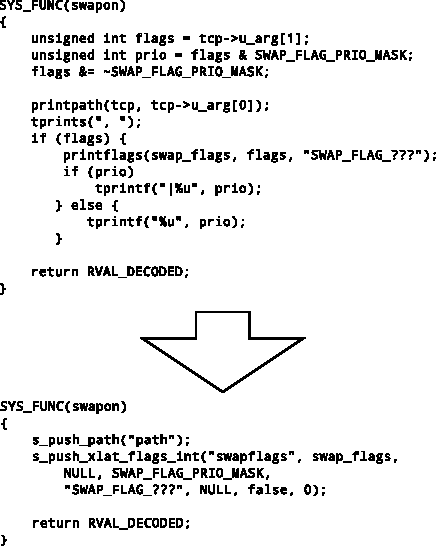
\includegraphics[width=1.0\textwidth]{lp0-conversion}
		\end{figure}
\end{columns}
\end{frame}

\begin{frame}{Structured output: illustration}
\begin{figure}[h]
      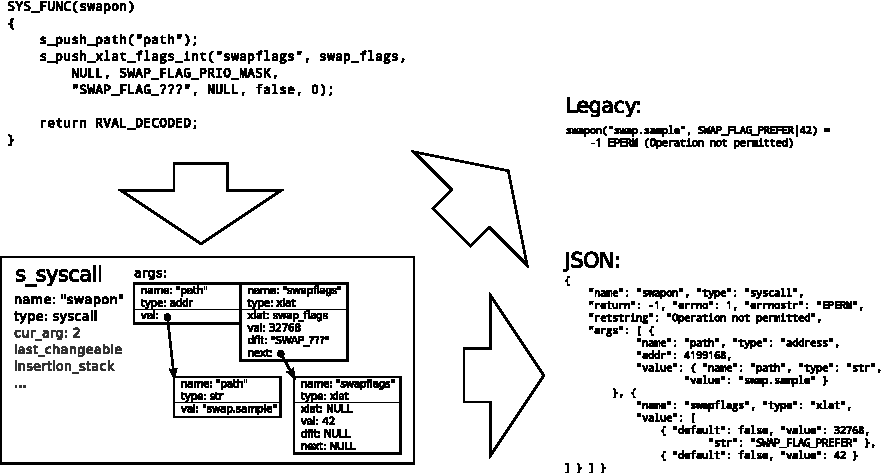
\includegraphics[width=\textwidth]{lp0-structured}
\end{figure}
\end{frame}

\begin{frame}[fragile]{Structured output: JSON output example}
\begin{scriptsize}
\begin{multicols}{2}
\begin{minted}{json}
{
    "name": "getrandom",
    "type": "syscall",
    "args": [
        {
            "name": "buf",
            "type": "changeable",
            "entering_value": null,
            "exiting_value": {
                "name": "buf",
                "type": "address",
                "addr": 140722827922048,
                "value": {
                    "name": "buf",
                    "type": "str",
                    "value": "\\x26\\x4d\\x4e",
                    "size": 3,
                    "truncated": true
                }
            }
        },
        {
            "name": "count",
            "value": 3
        },
        {
            "name": "flags",
            "type": "xlat",
            "value": [
                {
                    "default": true,
                    "value": 0
                }
            ]
        }
    ],
    "return": 3
}
\end{minted}
\end{multicols}
\end{scriptsize}
\end{frame}

%%%%%%%
\begin{frame}[fragile]{Advanced syscall filtering syntax}
\begin{block}{new syntax}
[\textbf{\textit{action(}}]\textbf{\textit{filter\_expression}}[;\textbf{\textit{arg1}}[;\textbf{\textit{arg2}}...]][)]
\begin{description}
\item[\textit{action}] is one of \textbf{trace}, \textbf{abbrev}, \textbf{verbose},
\textbf{raw}, \textbf{read}, \textbf{write}, \textbf{fault},
\textbf{inject}, or \textbf{stacktrace};
\item[\textit{arnN}] are arguments of \textbf{\textit{action}};
\item[\textit{filter\_expression}] is a combination of filters.
\end{description}
\end{block}
\begin{block}{supported filters}
\begin{description}
\item[syscall \textit{set}]: set of syscalls described by \textbf{\textit{set}};
\item[fd \textit{fd1}\dots]: set of syscalls operating with descriptor numbers
described by \textbf{\textit{fd1}}\dots;
\item[path \textit{path}]: set of syscalls operating with paths
described by \textbf{\textit{path}}.
\end{description}
\end{block}
\end{frame}

%%%%%%%
\begin{frame}[fragile]{Advanced syscall filtering syntax}
\begin{block}{echo -n foo | strace -e 'fd 1' cat >/dev/null}
\begin{small}
\begin{alltt}
fstat(1, {st_mode=S_IFCHR|0666, st_rdev=makedev(1, 3), ...}) = 0
write(1, "foo", 3)                      = 3
close(1)                                = 0
+++ exited with 0 +++
\end{alltt}
\end{small}
\end{block}
\begin{block}{strace -y -s4 -e 'syscall read' -e 'read(path /dev/zero)'  head -c5 /dev/zero}
\begin{small}
\begin{verbatim}
read(3</lib64/libc-2.26.so>, "\177ELF"..., 832) = 832
read(3</dev/zero>, "\0\0\0\0"..., 5)    = 5
 | 00000  00 00 00 00 00            .....            |
+++ exited with 0 +++
\end{verbatim}
\end{small}
\end{block}
\end{frame}

%%%%%%%
\begin{frame}[fragile]{Advanced syscall filtering syntax}
\begin{block}{strace -ve 'syscall \%file and not syscall \%desc' cat /dev/null}
\begin{small}
\begin{alltt}
execve("/bin/cat", ["/bin/cat", "/dev/null"], []) = 0
access("/etc/ld.so.preload", R_OK) = -1 ENOENT (No such file or directory)
+++ exited with 0 +++
\end{alltt}
\end{small}
\end{block}

\begin{block}{strace -ve 'syscall \%file and !(syscall \%desc || path /usr/bin/cat)' /bin/cat /dev/null}
\begin{small}
\begin{alltt}
strace: Requested path '/usr/bin/cat' resolved into '/bin/cat'
access("/etc/ld.so.preload", R_OK) = -1 ENOENT (No such file or directory)
+++ exited with 0 +++
\end{alltt}
\end{small}
\end{block}
\end{frame}

%%%%%%%
\begin{frame}[fragile]{Advanced syscall filtering syntax}
\begin{block}{strace -k -e 'fd 1' cat /dev/null}
\begin{small}
\begin{alltt}
fstat(1, {st_mode=S_IFCHR|0620, st_rdev=makedev(136, 5), ...}) = 0
 > /lib64/libc-2.24.so(__fxstat64+0x14) [0xdab54]
 > /bin/cat() [0x1bb9]
 > /lib64/libc-2.24.so(__libc_start_main+0xf0) [0x20400]
 > /bin/cat() [0x258b]
close(1)                                = 0
 > /lib64/libc-2.24.so(_IO_file_close+0xb) [0x7195b]
 > /lib64/libc-2.24.so(_IO_file_close_it+0x13c) [0x7302c]
 > /lib64/libc-2.24.so(fclose+0x1a3) [0x669a3]
 > /bin/cat() [0x5daa]
 > /bin/cat() [0x2a92]
 > /lib64/libc-2.24.so(__locale_getenv+0x140) [0x35c60]
 > /lib64/libc-2.24.so(exit+0x1a) [0x35cba]
 > /lib64/libc-2.24.so(__libc_start_main+0xf7) [0x20407]
 > /bin/cat() [0x258b]
+++ exited with 0 +++
\end{alltt}
\end{small}
\end{block}
\end{frame}

%%%%%%%
\begin{frame}[fragile]{Lua scripting}
\begin{block}{\large Advanced syscall tampering and filtering with Lua}
\begin{description}
\item[student]: Victor~Krapivensky
\item[mentors]: Eugene~Syromyatnikov, Dmitry~Levin
\end{description}
\end{block}
\begin{block}{Features available with Lua scripting}
\begin{itemize}
\item proper system call success injection
\item without breaking system call semantics
\item writing into tracee's memory
\end{itemize}
\end{block}
\end{frame}

%%%%%%%
\begin{frame}[fragile]{strace GSoC 2017 projects: Lua scripting}
\begin{alltt}
\scriptsize
$ uname
Linux
$ strace -l pretend.lua -qq -etrace=none uname
NeverMindOS

$ cat pretend.lua
ffi = require 'ffi'
f = assert(io.popen([[cpp - <<EOF | grep -v '^#'
#include <sys/utsname.h>
EOF]], 'r'))
ffi.cdef(f:read('*a'))
f:close()
assert(strace.hook('uname', 'exiting', function(tcp)
if tcp.u_rval == -1 then return end
local u = assert(strace.read_obj(tcp.u_arg[0], 'struct utsname'))
ffi.copy(u.sysname, 'NeverMindOS')
assert(strace.write_obj(tcp.u_arg[0], u))
end))
\end{alltt}
\end{frame}

%%%%%%%
\begin{frame}{strace GSoC 2017 projects: syscall information tool}
\begin{block}{\large Advanced syscall information tool}
\begin{description}
\item[student]: Edgar~Kaziakhmedov
\item[mentors]: Eugene~Syromyatnikov, Dmitry~Levin
\end{description}
\end{block}
\begin{block}{asinfo features}
\begin{itemize}
\item lists syscalls by various selection parameters,
e.g. number, name, group, and regex
\item processes any subset of many architectures supported by strace
\item prints in human-readable or script-friendly format
\end{itemize}
\end{block}
\end{frame}

%%%%%%%
\begin{frame}[fragile]{strace GSoC 2017 projects: syscall information tool}
\begin{alltt}
$ asinfo --set-arch x86\_64 --set-abi all --get-sname \%\%stat
|    |              | x86\_64 | x86\_64 | x86\_64 |
|  N | Syscall name |  64bit |    x32 |  32bit |
|  1 |        fstat |      5 |      5 |    108 |
|  2 |      fstat64 |      - |      - |    197 |
|  3 |    fstatat64 |      - |      - |    300 |
|  4 |        lstat |      6 |      6 |    107 |
|  5 |      lstat64 |      - |      - |    196 |
|  6 |   newfstatat |    262 |    262 |      - |
|  7 |     oldfstat |      - |      - |     28 |
|  8 |     oldlstat |      - |      - |     84 |
|  9 |      oldstat |      - |      - |     18 |
| 10 |         stat |      4 |      4 |    106 |
| 11 |       stat64 |      - |      - |    195 |
| 12 |        statx |    332 |    332 |    383 |
\end{alltt}
\end{frame}

%%%%%%%
\begin{frame}[fragile]{strace GSoC 2017 projects: syscall information tool}
\begin{alltt}
$ asinfo --set-arch x86_64 --set-abi all --get-sname /read
|    |                  | x86\_64 | x86\_64 | x86\_64 |
|  N |     Syscall name |  64bit |    x32 |  32bit |
|  1 |  get\_thread\_area |    211 |      - |    244 |
|  2 |          pread64 |     17 |     17 |    180 |
|  3 |           preadv |    295 |    534 |    333 |
|  4 |          preadv2 |    327 |    546 |    378 |
|  5 | process\_vm\_readv |    310 |    539 |    347 |
|  6 |             read |      0 |      0 |      3 |
|  7 |        readahead |    187 |    187 |    225 |
|  8 |          readdir |      - |      - |     89 |
|  9 |         readlink |     89 |     89 |     85 |
| 10 |       readlinkat |    267 |    267 |    305 |
| 11 |            readv |     19 |    515 |    145 |
| 12 |  set\_thread\_area |    205 |      - |    243 |
\end{alltt}
\end{frame}

%%%%%%%

\begin{frame}{Future ideas}
\begin{itemize}
	\item More elaborate parsers (especially for ioctls)
	\item More output formats (pcap-ng, CTF)
	\item Declarative syscall syntax description
	\item More tracing backends (EBPF)
	\item Better support for argument decoding in Lua (handling of structures in mpers)
	\item PID namespace translation
	\item Support for different target architectures (for gdbserver backend)
\end{itemize}
\end{frame}

{
\setbeamertemplate{logo}{}
\begin{frame}{Links}
\begin{columns}
	\column{10cm}
		\begin{block}{Project page}
			https://strace.io/
		\end{block}
		\begin{block}{strace.git}
			git://git.code.sf.net/p/strace/code.git

			https://github.com/strace/strace.git
		\end{block}
		\begin{block}{mailing list}
			strace-devel@lists.sourceforge.net
		\end{block}
		\begin{block}{\large IRC channel}
			\#strace@freenode
		\end{block}
	\column{4cm}
		\centerline{
\includegraphics[height=7cm]{strace.pdf}}
\end{columns}
\end{frame}
}

\end{document}
